\section{Élkonzisztencia algoritmusok}

\begin{definicio}
    Legyen $\mathcal{V}$ változók egy tetszőleges halmaza, $\mathcal{D}$ pedig
    egy olyan leképezés, amely minden $x \in \mathcal{V}$ változóhoz egy
    $\mathcal{D}(x)$-el jelölt halmazt (tartományt) rendel.

    Tetszőleges két különböző $x \in \mathcal{V}$ és $y \in \mathcal{V}$ változó
    közti bináris kényszer egy $\mathcal{D}(x)$ és $\mathcal{D}(y)$ feletti
    bináris reláció: \[
        R_{x,y} \subseteq  \mathcal{D}(x) \times \mathcal{D}(y)
    .\]

    Jelöljük $R^{-1}_{x,y}$ formában az $R_{x,y}$ reláció inverzét: \[
        R^{-1}_{x,y} = \{
            (b,a) : (a,b) \in R_{x,y}
        \}
    .\]
\end{definicio}

\begin{definicio}
    Véges, bináris kényszerkielégítési probléma.
    Egy {\bf véges, bináris kényszerkielégítése probléma} alatt olyan
    $\left<\mathcal{V}, \mathcal{D}, \mathcal{C} \right>$ rendezett hármast
    értünk, ahol
    \begin{itemize}
        \item $\mathcal{V}$ változók egy véges, nemüres halmaza
        \item $\mathcal{D}(x)$ minden $x \in \mathcal{V}$ változó esetén egy
            véges halmaz(tartomány)
        \item $\mathcal{C}$ a $\mathcal{V}$-beli változók feletti bináris
            kényszerek halmaza, úgy hogy
            \begin{itemize}
                \item ha $R_{x_y} \in \mathcal{C}$ és $R'_{x,y} \in
                    \mathcal{C}$ akkor $R_{x,y} = R'_{x,y}$.
                \item ha $R_{x_y} \in \mathcal{C}$ akkor $R_{y,x} \in
                    \mathcal{C}$ és $R_{y,x} = R^{-1}_{x,y}$.
            \end{itemize}
    \end{itemize}
\end{definicio}

\begin{definicio}
    Gráf reprezentáció.
    Egy $\left<\mathcal{V}, \mathcal{D}, \mathcal{C} \right>$(nem feltétlenül
    véges) {\bf bináris kényszerkielégítési probléma gráf reprezentációja}
    egy olyan $\left<N, E \right>$ pár, ahol:
    \begin{itemize}
        \item $N = \{n_v : v \in \mathcal{V}\}$ alkotja a gráf csúcsait,
        \item $E = \{
                (n_x, n_y) : R_{x,y} \in \mathcal{C}
            \}$ alkotja a gráf irányított éleit.
    \end{itemize}

    \begin{megjegyzes}
        Mivel $R_{x,y}$ és  $R_{y,x}$ bináris kényszerek ugyanazt fejezik ki,
        ezért az irányított élek helyett irányítatlan éleket tartalmazó gráfot
        szokás használni.

        Annak, hogy $R_{x,y}$ és  $R_{y,x}$ együtt szerepel a kényszerek között,
        a később bemutatott algoritmusokban lesz jelentősége.
    \end{megjegyzes}
\end{definicio}

\begin{definicio}
    Nem bináris kényszerek.

    {\bf Unáris kényszerek:} Az unáris kényszerek egyetlen változó értékét
    korlátoznák. A helyett, hogy ezt kényszerként jelenítenénk meg,
    kifejezhetjük azzal, hogy a változóhoz rendelt tartomány elemeiként eleve
    csak az unáris kényszernek megfelelő értékeket választunk.

    {\bf Magasabb rendű kényszerek:}  A magasabb rendű kényszerek mindig
    kiválthatók bináris kényszerekkel újabb változók bevezetése mellett.
\end{definicio}

\begin{definicio}
    Kényszerek terjesztése.
    A \textbf{kényszerek terjesztése} során egy tekintett változó értékére
    vonatkozó megszorítás következményeit a vele kényszerek útján kapcsolatban
    álló változók értékeire vonatkozóan is kiterjesztjük, ezen változók
    értékeire újabb megszorításokat alkalmazva.
\end{definicio}

\begin{definicio}
    Élkonzisztencia algoritmusok.
    Az \textbf{élkonzisztencia algoritmusok} feladata, a kényszerek
    terjesztésének hatékony megvalósítása. Ezen algoritmusok egyaránt
    alkalmazhatóak a keresés megkezdése előtt a probléma méretét csökkentő
    előfeldolgozó lépésként, vagy akár a keresés közben is. Ezek közül mi az
    előbbi lehetőséget vizsgáljuk meg.
\end{definicio}

\subsection{AC1}

Az AC-1 (gyakorlatban nem használt) algoritmus egyszerű naiv megközelítés
segítségével mutatja be a kényszerek terjesztésének ötletét.

\begin{definicio}
    Felülvizsgálat.
    Az $R_{x,y}$ \textbf{kényszer felülvizsgálat}a során a
    $\langle \mathcal{V}, \mathcal{D}, \mathcal{C} \rangle$
    bináris kényszereket tartalmazó véges kényszerkielégítési problémát a
    $\langle \mathcal{V}, \mathcal{D}', \mathcal{C}' \rangle$
    problémával helyettesítjük, ahol \[
    \mathcal{D}' =
    \begin{cases}
        \{a : a \in \mathcal{D}(x) \land b \in D(y) \land \langle a, b\rangle \in R_{x,y}\}
        &\text{ ha } z=x \\
        \mathcal{D}(z)
        &\text{ egyébként.}
    \end{cases}
    .\]
\end{definicio}

\begin{algorithm}[H]
    \Fn{\FACone{$\langle \mathcal{V}, \mathcal{D}, \mathcal{C} \rangle$}}
    {
        \Repeat{$\mathcal{D} = \mathcal{D}'$}{
            $\mathcal{D}' \gets \mathcal{D}$ \;
            \ForAll{$R_{x,y} \in \mathcal{C}$}
            {
                $\mathcal{D} \gets
                \revise\left(R_{x,y}, \langle \mathcal{V}, \mathcal{D},
                \mathcal{C} \rangle  \right)$
            }
        }
        \KwRet{$\langle \mathcal{V}, \mathcal{D}, \mathcal{C} \rangle$}\;
    }
    \caption{AC-1}
\end{algorithm}

\subsection{AC3}

Az AC-3 algoritmus (Mackworth) egy már a gyakorlatban is használható
algoritmus, amely egy sorban tartja nyilván azokat a kényszereket, amelyeket
felül kell vizsgálni.

Ha $R_{x,y}$ felülvizsgálat során az  $x$ változó tartománya megváltozik, akkor
minden olyan kényszer ismét bekerül a sorba, amely $R_{y,x}$ alakú.

Az algoritmus akkor fejeződik be, mikor elfogytak a sorból a kényszerek.

Az algoritmus időbonyolultsága $\mathcal{O}(n^2 \cdot d^3)$.

\begin{algorithm}[H]
    \Fn{\FACthree{$\langle \mathcal{V}, \mathcal{D}, \mathcal{C} \rangle$}}
    {
        \While{$W \neq \varnothing$}{
            remove an $R_{x,y}$ constraint from $W$\;
            $\mathcal{D}' \gets \mathcal{D}$ \;
            $\mathcal{D} \gets
            \revise\left(R_{x,y}, \langle \mathcal{V}, \mathcal{D},
            \mathcal{C} \rangle  \right)$\;
            \If{$\mathcal{D}' \neq \mathcal{D}$}{
                \eIf{$\mathcal{D}(x) = \varnothing$}{
                    \KwRet{failure}\;
                }{%
                    \ForAll{$R_{u,w} \in \{R_{u,w} : R_{u,w} \in
                        \mathcal{C} \land w = x\} $}{
                        $W \gets W \cup \{R_{u,w}\}$ \;
                    }
                }
            }
        }
        \KwRet{$\langle \mathcal{V}, \mathcal{D}, \mathcal{C} \rangle$}\;
    }
    \caption{AC-3}
\end{algorithm}

\subsection{AC4}

Az AC-4 algoritmus (Mohr és Henderson) két előre elkészített
adatszerkezettel dolgozik:

\begin{itemize}
    \item minden $R_{x,y}$ kényszer és $v_x \in  \mathcal{D}(x)$ értékhez egy
         számlálót rendelünk: \[
             C_{x,v_x,y} =
             \card \{v_y : v_y \in \mathcal{D}(y) \land \langle v_x, v_y \rangle \in R_{x,y}\}
         ,\]
     \item az $x$ változó minden $v_x \in \mathcal{D}(x)$ értékéhez egy halmazt
         rendelünk: \[
            S_{x,v_x} = \{
                \left<y, v_y \right> :
                v_y \in \mathcal{D}(y) \land
                \left<v_y, v_x \right> \in R_{y,x}
            \}
        ,\]
        amely megmutatja, hogy mely $y$ változók mely $v_y \in \mathcal{D}(y)$ értékeihez
        számoltuk hozzá $v_x$-et.
\end{itemize}

Jelölje $\mathcal{D}_{-\left<x, v_x \right>}$ azt a leképezést, amely
$\mathcal{D}$ leképezéstől annyiban különbözik, hogy $v_x \not\in
\mathcal{D}(x)$, vagyis $x$ nem veheti fel $v_x$ értéket: \[
    \mathcal{D}_{-\left<x, v_x \right>}(z) =
    \begin{cases}
        \mathcal{D}(x)\setminus \{v_x\} & \text{ ha } z=x,\\
        \mathcal{D}(z) & \text{ egyébként.}
    \end{cases}
\]

\begin{algorithm}[H]
    \Fn{\FACfourinit{$\langle \mathcal{V}, \mathcal{D}, \mathcal{C} \rangle$}}
    {
        Compute $S$ \;
        Compute $C$ \;
        \ForAll{$\left<x, v_x \right> \in \{\left<x, v_x \right> : C_{x,v_x,y}
            = 0\}$}{
            $\mathcal{D} \gets \mathcal{D}_{-\left<x, v_x \right>}$
        }
        \KwRet{$S, C, \mathcal{D}$}\;
    }
    \caption{AC-4 inicializálás}
\end{algorithm}

\begin{algorithm}[H]
    \Fn{\FACfour{$\langle \mathcal{V}, \mathcal{D}, \mathcal{C} \rangle$}}
    {
        $S, C, D \gets$ \FACfourinit{$\left< \mathcal{V}, \mathcal{D},
        \mathcal{C} \right>$} \;

        $W \gets \{\left<x, v_x \right> : C_{x,v_x,y} = 0\} $

        \While{$W \neq \varnothing$}{
            remove an $\left<x,v_x \right>$ pair from $W$ \;
            \ForAll{$\left<y, v_y \right> \in S_{x, v_x}$}{
                $C_{y, v_y, x} \gets C_{y, v_y, x} - 1$ \;
                \If{$C_{y, v_y, x} = 0$ \textbf{and} $v_y \in \mathcal{D}_y$}
                {
                $\mathcal{D} \gets \mathcal{D}_{-\left<y, v_y \right>}$ \;
                insert the $\left<y, v_y \right>$ pair into $W$\;
                }
            }
        }
        \KwRet{$S, C, \mathcal{D}$}\;
    }
    \caption{AC-4}
\end{algorithm}

Az {\bf AC-4 algoritmus} egy váltótó-érték párokat tartalmazó munkahalmaz
segítségével végzi el feladatát. Azon értékek, amelyek által $C$ számlálója $0$-ra
csökken törölni kell a változó tartományából. A munkahalmazba a törtölt értékek
kerülnek, mert a tőlük függő értékek számlálóit csökkenteni kell. Ezek gyors
felderítésében segít $S$.

\begin{megjegyzes}
    Az AC-4 algoritmus időbonyolultsága: $\mathcal{O}(n^2 \cdot d^2)$. Ennek ellenére valódi
    problémák esetében sok esetben az AC-3 algoritmus teljesít jobban (Richard
    J.  Wallace).
\end{megjegyzes}

\subsection{Visszalépéses kereső}

\begin{figure}[H]
    \centering
    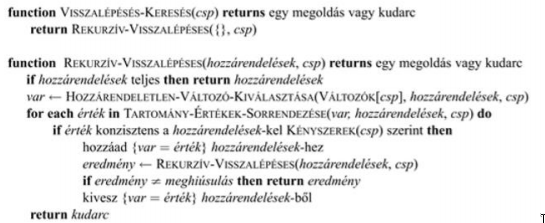
\includegraphics[width=0.8\textwidth]{visszalep}
    \caption{Visszalépéses kereső algoritmusa}
    \label{fig:visszalep}
\end{figure}
